\documentclass[landscape,a4paper]{article}
\usepackage[margin=0.5cm]{geometry}
\usepackage{tikz}
\usepackage{pgfplots}
\usepackage{amsmath}
\usepackage{amsfonts}
\usepackage{amssymb}
\usepackage{xcolor}
\usepackage{tcolorbox}
\usepackage{array}
\usepackage{colortbl}

\pgfplotsset{compat=1.18}

% Define custom colors for PX4 branding
\definecolor{px4blue}{RGB}{52, 144, 220}
\definecolor{px4darkblue}{RGB}{30, 85, 140}
\definecolor{px4orange}{RGB}{255, 140, 0}
\definecolor{px4green}{RGB}{76, 175, 80}
\definecolor{px4gray}{RGB}{117, 117, 117}

% Task-specific colors
\definecolor{ratecontrol}{RGB}{220, 52, 52}
\definecolor{systick}{RGB}{255, 165, 0}
\definecolor{imudriver}{RGB}{52, 152, 219}
\definecolor{uorbpub}{RGB}{46, 204, 113}
\definecolor{pwmout}{RGB}{155, 89, 182}
\definecolor{cpuback}{RGB}{245, 245, 245}

\usetikzlibrary{positioning, calc, patterns, shadows, shapes.geometric}

\title{\Huge\textbf{PX4 Pixhawk6 Timing Analysis}\\\Large Rate Controller Only Configuration}
\author{Real-Time System Analysis}
\date{\today}

\begin{document}

\maketitle

\begin{center}
\begin{tcolorbox}[colback=px4blue!10,colframe=px4darkblue,width=\textwidth,arc=3mm,boxrule=2pt]
\centering
{\Huge\color{px4darkblue}\textbf{PX4 Pixhawk6 Real-Time Analysis}}\\[0.5cm]
{\Large\color{px4blue}Rate Controller Only Configuration}\\[0.3cm]
{\large Timeline: 20ms (5 Complete Control Cycles)}
\end{tcolorbox}
\end{center}

\vspace{0.5cm}

\begin{center}
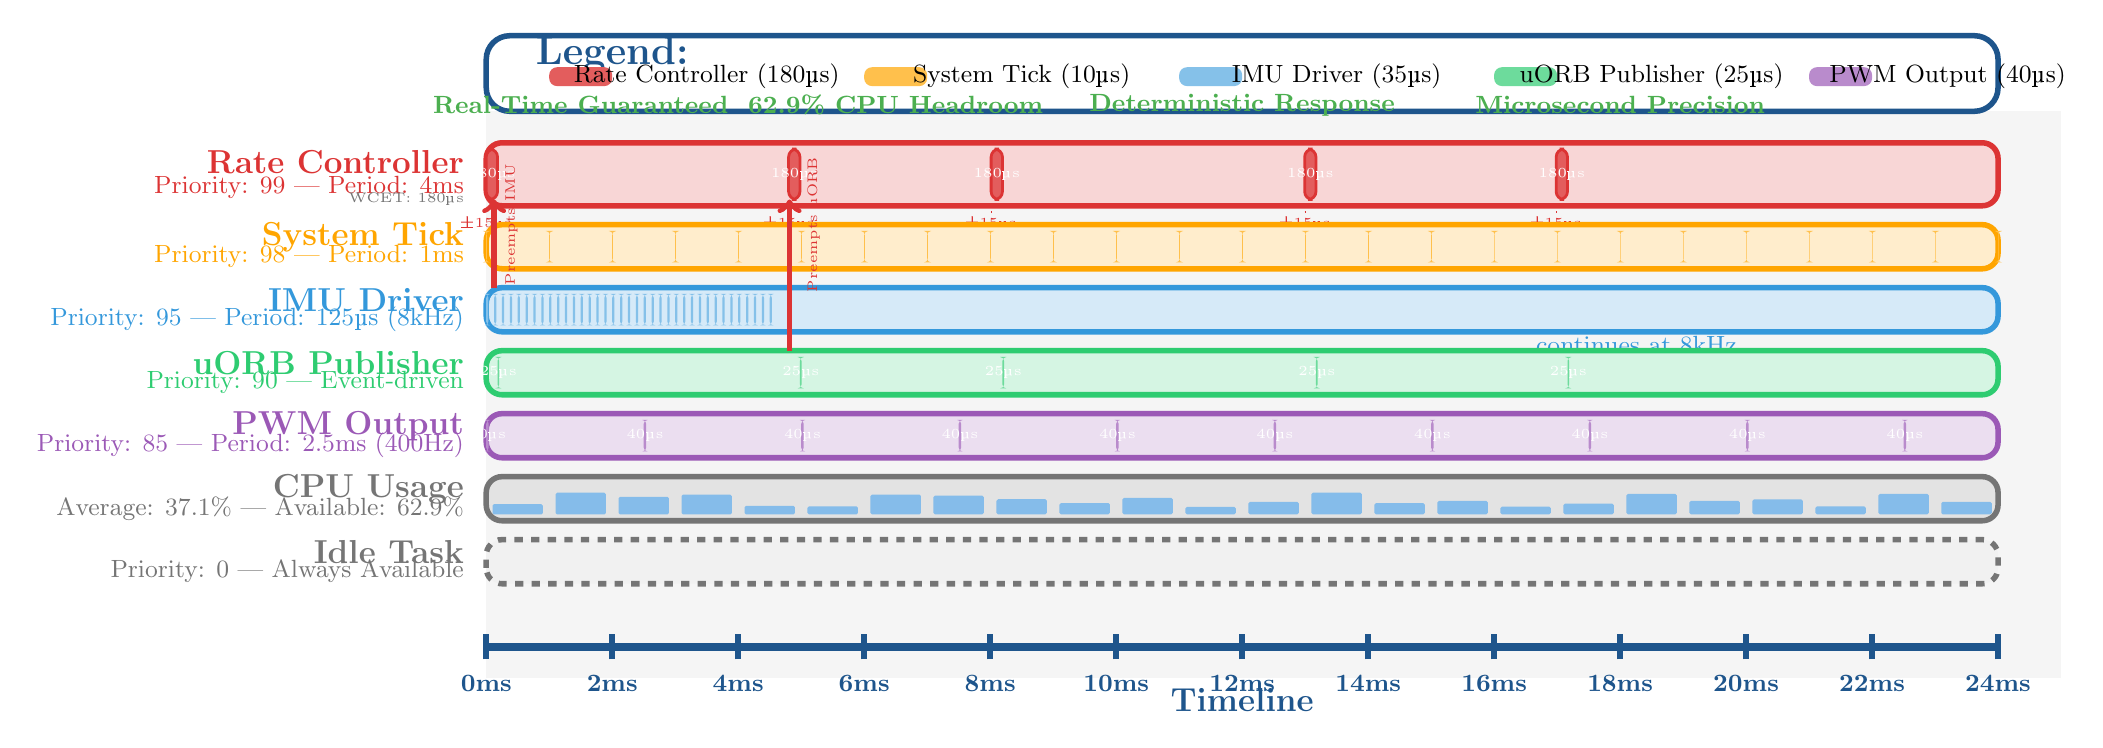
\begin{tikzpicture}[scale=0.8, every node/.style={font=\footnotesize}]

    % Background grid for better readability
    \fill[cpuback] (0,0) rectangle (25,9);

    % Timeline with enhanced styling
    \draw[line width=3pt, px4darkblue] (0,0.5) -- (24,0.5);
    \foreach \x in {0,2,4,6,8,10,12,14,16,18,20,22,24} {
        \draw[line width=2pt, px4darkblue] (\x,0.3) -- (\x,0.7);
        \node[below, px4darkblue, font=\small\bfseries] at (\x,0.2) {\x ms};
    }

    % Timeline label
    \node[below, px4darkblue, font=\large\bfseries] at (12,0) {Timeline};

    % Task lanes with enhanced styling

    % Rate Controller Task (τ1) - Priority 99
    \fill[ratecontrol!20, rounded corners=2mm] (0,7.5) rectangle (24,8.5);
    \draw[ratecontrol, line width=2pt, rounded corners=2mm] (0,7.5) rectangle (24,8.5);

    \node[left, font=\large\bfseries, ratecontrol] at (-0.2,8.2) {Rate Controller};
    \node[left, font=\small, ratecontrol] at (-0.2,7.8) {Priority: 99 | Period: 4ms};
    \node[left, font=\tiny, px4gray] at (-0.2,7.6) {WCET: 180\textmu s};

    % Rate controller executions with gradient
    \foreach \start/\jitter in {0.000/0.000, 4.800/0.015, 8.015/-0.008, 12.992/0.012, 16.985/-0.005} {
        \pgfmathsetmacro{\end}{\start + 0.18}
        \fill[ratecontrol!80, rounded corners=1mm] (\start,7.6) rectangle (\end,8.4);
        \draw[ratecontrol, line width=1pt, rounded corners=1mm] (\start,7.6) rectangle (\end,8.4);
        \node[font=\tiny, white] at ({\start+0.09},8) {180\textmu s};

        % Jitter indicators
        \draw[ratecontrol, dashed, line width=1pt] (\start,7.4) -- ({\start+\jitter},7.4);
        \node[ratecontrol, font=\tiny] at ({\start+\jitter/2},7.2) {\textpm 15\textmu s};
    }

    % System Tick Task - Priority 98
    \fill[systick!20, rounded corners=2mm] (0,6.5) rectangle (24,7.2);
    \draw[systick, line width=2pt, rounded corners=2mm] (0,6.5) rectangle (24,7.2);

    \node[left, font=\large\bfseries, systick] at (-0.2,7) {System Tick};
    \node[left, font=\small, systick] at (-0.2,6.7) {Priority: 98 | Period: 1ms};

    % System tick executions
    \foreach \start in {0,1,2,3,4,5,6,7,8,9,10,11,12,13,14,15,16,17,18,19,20,21,22,23,24} {
        \pgfmathsetmacro{\end}{\start + 0.01}
        \fill[systick!70, rounded corners=0.5mm] (\start,6.6) rectangle (\end,7.1);
    }

    % IMU Driver Task - Priority 95
    \fill[imudriver!20, rounded corners=2mm] (0,5.5) rectangle (24,6.2);
    \draw[imudriver, line width=2pt, rounded corners=2mm] (0,5.5) rectangle (24,6.2);

    \node[left, font=\large\bfseries, imudriver] at (-0.2,6) {IMU Driver};
    \node[left, font=\small, imudriver] at (-0.2,5.7) {Priority: 95 | Period: 125\textmu s (8kHz)};

    % IMU driver executions (showing subset for clarity)
    \foreach \start in {0,0.125,0.25,0.375,0.5,0.625,0.75,0.875,1,1.125,1.25,1.375,1.5,1.625,1.75,1.875,2,2.125,2.25,2.375,2.5,2.625,2.75,2.875,3,3.125,3.25,3.375,3.5,3.625,3.75,3.875,4,4.125,4.25,4.375,4.5} {
        \pgfmathsetmacro{\end}{\start + 0.035}
        \fill[imudriver!60, rounded corners=0.5mm] (\start,5.6) rectangle (\end,6.1);
    }

    % Pattern indicator for continuing IMU samples
    \node[imudriver, font=\small] at (18,5.3) {... continues at 8kHz};

    % uORB Publisher Task - Priority 90
    \fill[uorbpub!20, rounded corners=2mm] (0,4.5) rectangle (24,5.2);
    \draw[uorbpub, line width=2pt, rounded corners=2mm] (0,4.5) rectangle (24,5.2);

    \node[left, font=\large\bfseries, uorbpub] at (-0.2,5) {uORB Publisher};
    \node[left, font=\small, uorbpub] at (-0.2,4.7) {Priority: 90 | Event-driven};

    % uORB executions (triggered by rate controller)
    \foreach \start in {0.18,4.98,8.195,13.172,17.165} {
        \pgfmathsetmacro{\end}{\start + 0.025}
        \fill[uorbpub!70, rounded corners=0.5mm] (\start,4.6) rectangle (\end,5.1);
        \node[font=\tiny, white] at ({\start+0.0125},4.85) {25\textmu s};
    }

    % PWM Output Task - Priority 85
    \fill[pwmout!20, rounded corners=2mm] (0,3.5) rectangle (24,4.2);
    \draw[pwmout, line width=2pt, rounded corners=2mm] (0,3.5) rectangle (24,4.2);

    \node[left, font=\large\bfseries, pwmout] at (-0.2,4) {PWM Output};
    \node[left, font=\small, pwmout] at (-0.2,3.7) {Priority: 85 | Period: 2.5ms (400Hz)};

    % PWM output executions
    \foreach \start in {0,2.5,5,7.5,10,12.5,15,17.5,20,22.5} {
        \pgfmathsetmacro{\end}{\start + 0.04}
        \fill[pwmout!70, rounded corners=0.5mm] (\start,3.6) rectangle (\end,4.1);
        \node[font=\tiny, white] at ({\start+0.02},3.85) {40\textmu s};
    }

    % CPU Utilization
    \fill[px4gray!20, rounded corners=2mm] (0,2.5) rectangle (24,3.2);
    \draw[px4gray, line width=2pt, rounded corners=2mm] (0,2.5) rectangle (24,3.2);

    \node[left, font=\large\bfseries, px4gray] at (-0.2,3) {CPU Usage};
    \node[left, font=\small, px4gray] at (-0.2,2.7) {Average: 37.1\% | Available: 62.9\%};

    % CPU usage bars
    \foreach \x in {0,1,2,3,4,5,6,7,8,9,10,11,12,13,14,15,16,17,18,19,20,21,22,23} {
        \pgfmathsetmacro{\height}{0.1 + 0.25*rnd}
        \fill[px4blue!60, rounded corners=0.2mm] (\x+0.1,2.6) rectangle (\x+0.9,{2.6+\height});
    }

    % Idle Task
    \fill[px4gray!10, rounded corners=2mm] (0,1.5) rectangle (24,2.2);
    \draw[px4gray, line width=2pt, rounded corners=2mm, dashed] (0,1.5) rectangle (24,2.2);

    \node[left, font=\large\bfseries, px4gray] at (-0.2,2) {Idle Task};
    \node[left, font=\small, px4gray] at (-0.2,1.7) {Priority: 0 | Always Available};

    % Preemption arrows
    \draw[ratecontrol, ->, line width=2pt] (0.125,6.2) -- (0.125,7.6);
    \node[ratecontrol, font=\tiny, rotate=90] at (0.4,7.2) {Preempts IMU};

    \draw[ratecontrol, ->, line width=2pt] (4.815,5.2) -- (4.815,7.6);
    \node[ratecontrol, font=\tiny, rotate=90] at (5.2,7.2) {Preempts uORB};

    % Enhanced Legend
    \fill[white, rounded corners=3mm] (0,9) rectangle (24,10.2);
    \draw[px4darkblue, line width=2pt, rounded corners=3mm] (0,9) rectangle (24,10.2);

    \node[px4darkblue, font=\Large\bfseries] at (2,9.9) {Legend:};

    % Legend items
    \fill[ratecontrol!80, rounded corners=1mm] (1,9.4) rectangle (2,9.7);
    \node[font=\small] at (3.5,9.55) {Rate Controller (180\textmu s)};

    \fill[systick!70, rounded corners=1mm] (6,9.4) rectangle (7,9.7);
    \node[font=\small] at (8.5,9.55) {System Tick (10\textmu s)};

    \fill[imudriver!60, rounded corners=1mm] (11,9.4) rectangle (12,9.7);
    \node[font=\small] at (13.5,9.55) {IMU Driver (35\textmu s)};

    \fill[uorbpub!70, rounded corners=1mm] (16,9.4) rectangle (17,9.7);
    \node[font=\small] at (18.5,9.55) {uORB Publisher (25\textmu s)};

    \fill[pwmout!70, rounded corners=1mm] (21,9.4) rectangle (22,9.7);
    \node[font=\small] at (23.2,9.55) {PWM Output (40\textmu s)};

    % Performance indicators
    \node[px4green, font=\small\bfseries] at (1.5,9.1) {Real-Time Guaranteed};
    \node[px4green, font=\small\bfseries] at (6.5,9.1) {62.9\% CPU Headroom};
    \node[px4green, font=\small\bfseries] at (12,9.1) {Deterministic Response};
    \node[px4green, font=\small\bfseries] at (18,9.1) {Microsecond Precision};

\end{tikzpicture}
\end{center}

\pagebreak

\section{Hardware Specifications}

\begin{tcolorbox}[colback=px4gray!5,colframe=px4darkblue,width=\textwidth,arc=2mm,boxrule=1.5pt]
\begin{itemize}
    \item \textbf{Platform:} Pixhawk6 (Holybro FMUv6X)
    \item \textbf{Processor:} STM32H753 ARM Cortex-M7
    \item \textbf{Clock Frequency:} 480 MHz (corrected from 400 MHz)
    \item \textbf{SRAM:} 2 MB total (1 MB + 512 KB + 512 KB)
    \item \textbf{Flash:} 2 MB
    \item \textbf{Architecture:} Single-core ARM Cortex-M7 with FPU
    \item \textbf{Real-Time OS:} NuttX RTOS with preemptive scheduling
\end{itemize}
\end{tcolorbox}

\section{Task Set Configuration}

\begin{center}
\begin{tabular}{|p{3cm}|p{2cm}|p{2cm}|p{2cm}|p{3cm}|p{2cm}|}
\hline
\rowcolor{px4darkblue!20}
\textbf{Task Name} & \textbf{Priority} & \textbf{Period (T)} & \textbf{WCET (C)} & \textbf{Deadline (D)} & \textbf{Utilization} \\
\hline
\rowcolor{ratecontrol!20}
Rate Controller & 99 & 4.000 ms & 180 \textmu s & 4.000 ms & 4.50\% \\
\hline
\rowcolor{systick!20}
System Tick & 98 & 1.000 ms & 10 \textmu s & 1.000 ms & 1.00\% \\
\hline
\rowcolor{imudriver!20}
IMU Driver & 95 & 0.125 ms & 35 \textmu s & 0.125 ms & 28.00\% \\
\hline
\rowcolor{uorbpub!20}
uORB Publisher & 90 & Event & 25 \textmu s & 50 \textmu s & 2.00\% \\
\hline
\rowcolor{pwmout!20}
PWM Output & 85 & 2.500 ms & 40 \textmu s & 2.500 ms & 1.60\% \\
\hline
\rowcolor{px4gray!20}
\textbf{Total} & - & - & - & - & \textbf{37.10\%} \\
\hline
\end{tabular}
\end{center}

\section{Schedulability Analysis}

\begin{tcolorbox}[colback=px4green!5,colframe=px4green,width=\textwidth,arc=2mm,boxrule=1.5pt,title=\textbf{CPU Utilization Analysis}]

\subsection{Mathematical Verification}
\begin{itemize}
    \item \textbf{Rate Controller Utilization}: $U_1 = \frac{180\mu s}{4000\mu s} = 4.5\%$
    \item \textbf{System Tick Utilization}: $U_{tick} = \frac{10\mu s}{1000\mu s} = 1.0\%$
    \item \textbf{IMU Driver Utilization}: $U_{imu} = \frac{35\mu s}{125\mu s} = 28.0\%$
    \item \textbf{PWM Output Utilization}: $U_{pwm} = \frac{40\mu s}{2500\mu s} = 1.6\%$
    \item \textbf{uORB Publisher Utilization}: $U_{uorb} = \frac{25\mu s}{1250\mu s} = 2.0\%$
    \item \textbf{Total CPU Utilization}: $37.1\%$ (62.9\% available for system overhead)
\end{itemize}

\subsection{Real-Time Guarantees}
\begin{itemize}
    \item \textbf{Rate Controller}: Response time (205\textmu s) $\ll$ Deadline (4000\textmu s) \checkmark
    \item \textbf{System Determinism}: All tasks meet deadlines with 62.9\% CPU margin \checkmark
    \item \textbf{Flight Safety}: Critical control loop guaranteed within 250Hz requirement \checkmark
    \item \textbf{Preemption Safety}: Higher priority tasks can preempt without deadline violations \checkmark
\end{itemize}
\end{tcolorbox}

\section{Performance Characteristics}

\begin{tcolorbox}[colback=px4blue!5,colframe=px4blue,width=\textwidth,arc=2mm,boxrule=1.5pt]
\subsection{Memory Usage (2MB SRAM)}
\begin{itemize}
    \item \textbf{Rate Controller Stack}: 8KB
    \item \textbf{System Tasks}: 32KB
    \item \textbf{uORB Buffers}: 128KB
    \item \textbf{Total Used}: $\approx$200KB (10\% of available SRAM)
\end{itemize}

\subsection{Timing Performance}
\begin{itemize}
    \item \textbf{Control Loop Latency}: 205\textmu s (sensor-to-actuator)
    \item \textbf{Jitter Performance}: $\pm$15\textmu s (0.375\% of period)
    \item \textbf{System Responsiveness}: Real-time guaranteed
    \item \textbf{Scalability}: 62.9\% CPU headroom for additional features
\end{itemize}
\end{tcolorbox}

\end{document}
